% Latex Beamer template following CERN template guidelines (or trying!)

\documentclass[14pt,aspectratio=169]{beamer}
\usepackage{xcolor}
\usepackage{graphicx}
\usepackage{multicol}
\usepackage{tikz}
\usepackage[utf8]{inputenc}
\usepackage{xcolor}
\usepackage{moresize}

% Code listings with syntax highlighting
%  Require Pygments
\usepackage[outputdir=build]{minted}

\usetheme{cern}

% \newcommand{\interludeTitle}{We are here!}
% \AtBeginSection[] {
%   \frame{
%     \frametitle{\interludeTitle}
%     \begin{multicols}{2}
%       \tableofcontents[
%         currentsection,
%         sectionstyle=show/shaded,
%       ]
%     \end{multicols}
%   }
% }

% \AtBeginSubsection[] {
%   \frame{
%     \frametitle{\interludeTitle}
%     \begin{multicols}{2}
%       \tableofcontents[
%         currentsubsection,
%         sectionstyle=show/shaded,
%         subsectionstyle=show/shaded,
%       ]
%     \end{multicols}
%   }
% }


% Talk date
% Uncomment this to define a presentation date distinct from \today
\def\mydate{1 May 2019}

% Preamble
\title[]{Docker image testing in GitLab CI}
%% \subtitle{(no subtitle..)}
%\author[Author]{\texorpdfstring{\url{thomas.loekkeborg@cern.ch}}{Author}}
\author[Author]{Thomas Løkkeborg - IT-DB-DAR}

% Body
\begin{document}

\cernSplashBlue

% Title
{
  \setbeamertemplate{footline}{}
  \setbeamertemplate{navigation symbols}{}
  \frame{\titlepage}
}
\setcounter{framenumber}{0}

% TOC
\frame{
  \frametitle{Outline}
  \begin{multicols}{2}
    \tableofcontents
  \end{multicols}
}


\section{Introduction}

\subsection{Features used}

\begin{frame}
  \frametitle{Features used}
    \begin{itemize}
      \item GitLab CI
      \begin{itemize}
        \item Private GitLab Runners
        \begin{itemize}
          \item \mintinline{bash}{--privileged}
        \end{itemize}
        \item Docker-in-Docker
        \begin{itemize}
          \item docker:dind -> \mintinline{yaml}{alias: localhost}
          \item \mintinline{bash}{--cache-from}
        \end{itemize}
        \item Artifacts
        \begin{itemize}
          \item \mintinline{bash}{docker save / load} = tarball
        \end{itemize}
        \item GitLab Runner Exec
      \end{itemize}
      \item GitLab Container Registry
    \end{itemize}
  \begin{figure}
    
\includegraphics[width=0.3\textwidth]{images/gitlab.png}
  \end{figure}
\end{frame}

\subsection{The pipeline}

\begin{frame}
  \frametitle{The Pipeline*}
  \begin{figure}
    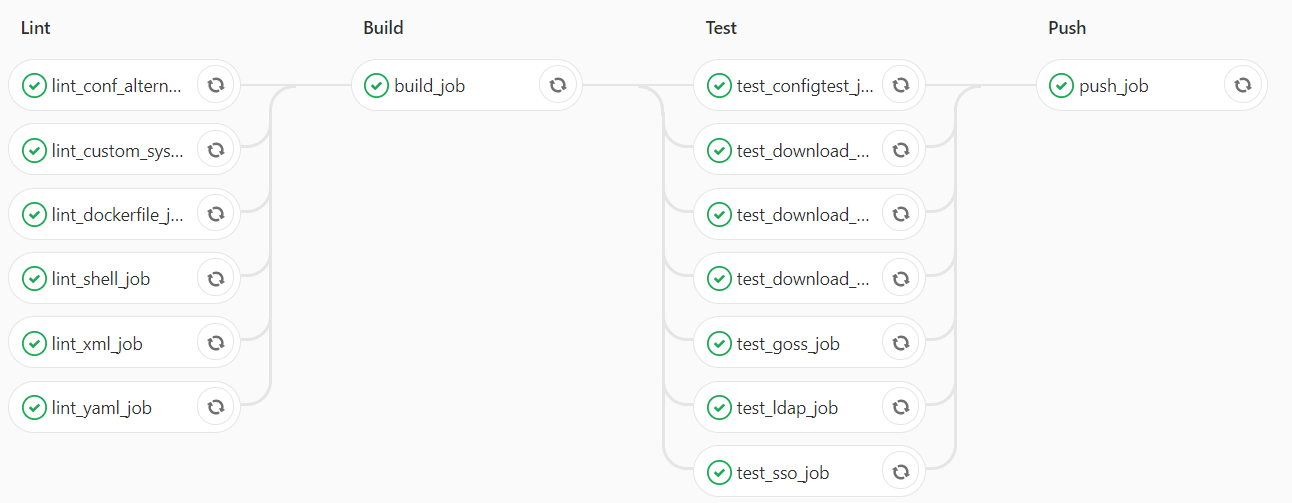
\includegraphics[width=\textwidth]{images/pipeline_2.png}
  \end{figure}
\end{frame}

\begin{frame}
  \frametitle{The Pipeline}
  \begin{figure}
    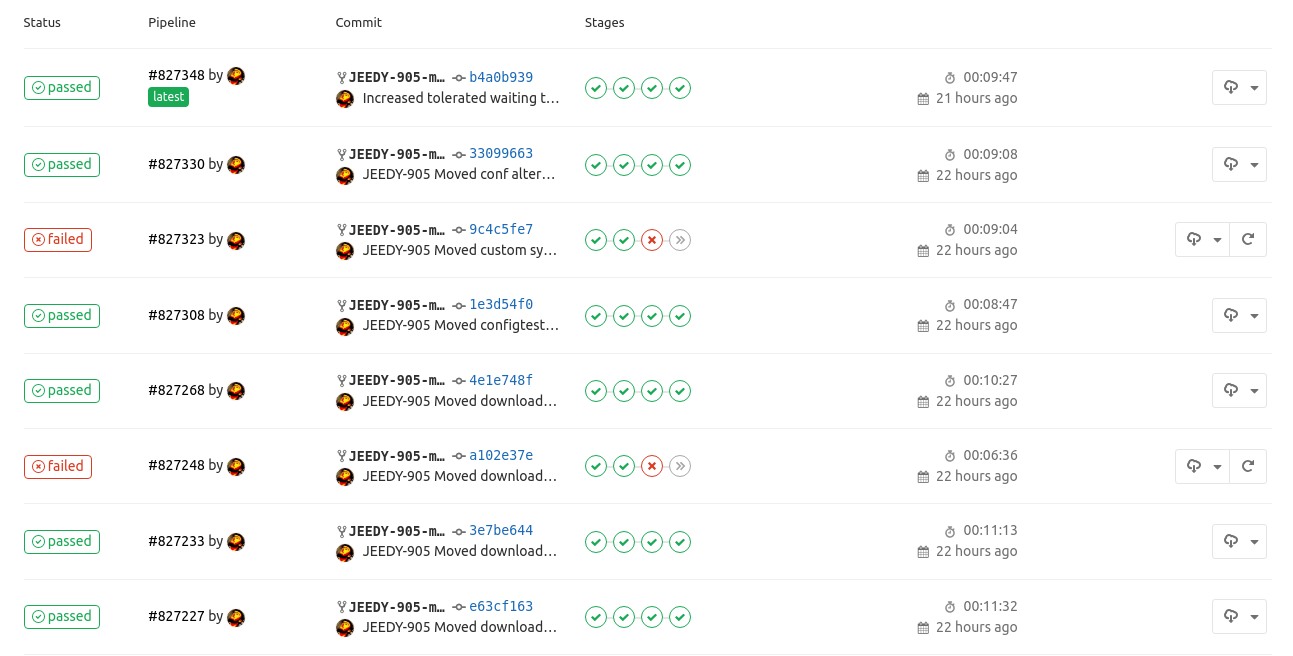
\includegraphics[width=0.8\textwidth]{images/pipeline_list.png}
  \end{figure}
\end{frame}

\begin{frame}
  \frametitle{The Pipeline - Quick facts}
  \begin{itemize}
    \item Aprox. duration of full pipeline: 13 minutes
    \item Jobs per pipeline: 26
    \item Total pipelines: 351
    \item Success rate: 79\%
    \item Biggest timestealer: Passing artifacts + \mintinline{bash}{docker save/load}
  \end{itemize}
\end{frame}

\subsection{General approach}

\begin{frame}
  \frametitle{General approach to writing tests}
  \textit{TODO / TOberemoved}
  \begin{itemize}
    \item Should run both in pipeline and locally
  \end{itemize}
\end{frame}

\section{The Tests}

\subsection{Goss}

% fragile cause verbatim used
\begin{frame}[fragile]
  \frametitle{Goss - Dgoss}
  \begin{itemize}
    \item Asserts Docker image meets requirements described in goss.yaml file
    \item Can generate goss.yaml from running container
  \end{itemize}

  \begin{minted}[
      frame=topline,
      fontsize=\tiny,
      breaklines,
    ]{yaml}
user:
  tomcat:
    uid: 1000
    gid: 1000
    exists: true
    groups:
      - tomcat
    shell: /sbin/nologin
http:
  http://localhost:8080/health-check/:
    status: 200
    no-follow-redirects: true
    timeout: 5000
    body:
      - I'm running
  \end{minted}
\end{frame}

% fragile cause verbatim used
\begin{frame}[fragile]
  \frametitle{Goss - Example}
  \begin{minted}[
      frame=bottomline,
      fontsize=\scriptsize,
      breaklines,
    ]{bash}
    GOSS_FILES_PATH=tests GOSS_FILES_STRATEGY=cp GOSS_SLEEP=5 dgoss run -e SOME_VAR=some-value -v /mount/path/outer:/mount/path/inner image-under-test
  \end{minted}
  \begin{figure}
    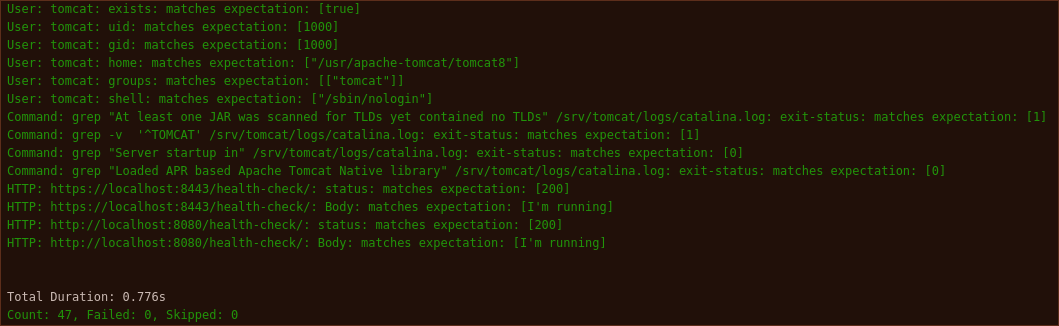
\includegraphics[width=\textwidth]{images/goss.png}
  \end{figure}
\end{frame}


\subsection{SSO}

\begin{frame}
  \frametitle{SSO Test - Concept} 
  \begin{itemize}
    \item «Given valid webapp and idP, can a test user log in successfully?»
    \item Keycloak as containerized idP with test data from JSON
    \item Webapp that shows received information about logged-in user
    \item Steps:
    \begin{itemize}
      \item Setup - Start containers
      \item Execute - Perform test
      \item Teardown - Remove containers and dump logs
    \end{itemize}
  \end{itemize}
  \begin{figure}
    
\includegraphics[width=0.3\textwidth]{images/keycloak_logo.png}
  \end{figure}
\end{frame}

% fragile cause verbatim used
\begin{frame}[fragile]
  \frametitle{SSO Test - Setup}

  \begin{minted}[
      fontsize=\scriptsize,
      breaklines,
    ]{bash}
docker run \
 --name=sso-test-tomcat-container \
 -d \
 -p 8080:8080 \
 -e JEEDY_TOMCAT_SSO_IDP_LOGIN_BINDING_URL=\
    http://localhost:9090/auth/realms/testrealm/protocol/saml \
 -e JEEDY_TOMCAT_SSO_ENTITY_ID=sample-webapp-entity-id \
 -v "$PWD"/tests/sso/web.xml:/srv/tomcat/webapps/sample/WEB-INF/web.xml \
 test-image

docker run \
 --name=sso-test-keycloak-container \
 -d \
 -p 9090:8080 \
 -v "$PWD"/tests/sso/testrealm.json:/tmp/testrealm.json \
 -e KEYCLOAK_IMPORT=/tmp/testrealm.json \
 -e KEYCLOAK_USER=admin \
 -e KEYCLOAK_PASSWORD=admin \
 "${KEYCLOAK_IMAGE}"
  \end{minted}
\end{frame}

\begin{frame}
  \frametitle{SSO Test - Execute}
  \begin{itemize}
    \item Curl application and expect redirect to Keycloak log-in
    \item Curl log-in form to Keycloak and receive SAMLResponse
    \item Manually POST SAMLResponse to application (would be done by JavaScript)
    \item Assert that application recieved information we expected
  \end{itemize}
\end{frame}

\begin{frame}
  \frametitle{SSO Test - Teardown}
  \begin{itemize}
    \item Remove containers
    \item Dump container logs
  \end{itemize}
\end{frame}

\subsection{LDAP}

% fragile because contains verbatim
\begin{frame}[fragile]
  \frametitle{LDAP Test}
  \begin{itemize}
    \item Follows structure of SSO test
    \item Containerized LDAP server with test data
  \end{itemize}
  \begin{minted}[
      frame=topline,
      fontsize=\fontsize{7pt}{7pt},
      breaklines,
    ]{bash}
do_curl_test_with_basic_auth \
 "fakeuser:fakepassword" \
 "401" \
 "fake user 'fakeuser' should not be able to authenticate"

do_curl_test_with_basic_auth \
 "testuser1:fakepassword" \
 "401" \
 "valid user 'testuser1' should not be able to authenticate with an invalid password"

do_curl_test_with_basic_auth \
 "testuser1:testpassword1" \
 "200" \
 "valid user 'testuser1' should be authorized to access the webapp due to nested e-groups"

do_curl_test_with_basic_auth \
 "testuser2:testpassword2" \
 "403" \
 "valid user 'testuser2' should not be authorized to access the webapp"
  \end{minted}
\end{frame}


\subsection{Building multiple images}

% fragile cause contains verbatim
\begin{frame}[fragile]
  \frametitle{Building multiple versions of image}
  \begin{itemize}
    \item GitLab CI missing "build matrix" feature
    \begin{itemize}
      \item Anchors/References
      \item Extends/Include
    \end{itemize}
  \end{itemize}
  \begin{minted}[
      frame=topline,
      fontsize=\scriptsize,
      breaklines,
    ]{yaml}
job_build_8_5_jdk7:
  variables:
    <<: *template_reference_common_variables_docker_dind
    <<: *template_reference_tomcat_8_5_jdk7_variables
  <<: *template_reference_build

job_build_9_0_jdk8:
  variables:
    <<: *template_reference_common_variables_docker_dind
    <<: *template_reference_tomcat_9_0_jdk8_variables
  <<: *template_reference_build
  \end{minted}
\end{frame}

% fragile cause contains verbatim
\begin{frame}[fragile]
  \frametitle{The templates - YAML anchors/references 101}
  \begin{minted}[
      fontsize=\small,
      breaklines,
    ]{yaml}
.hidden: &anchor
  image: docker:18-09

my_job:
  # reference to anchor
  <<: *anchor
  script:
    - docker info
  \end{minted}
\end{frame}

% fragile cause contains verbatim
\begin{frame}[fragile]
  \frametitle{The templates - Common all DinD jobs}
  \begin{minted}[
      fontsize=\scriptsize,
      breaklines,
    ]{yaml}
.template_common_all_docker_dind_jobs: &template_reference_common_all_docker_dind_jobs
  image: docker:18.09
  tags:
    - db-runner-docker-privilege
  before_script:
    - docker info
    - docker login -u gitlab-ci-token -p $CI_BUILD_TOKEN $CI_REGISTRY
    - if [ -z $RUNNING_LOCALLY ]; then ln -s "$PWD" /artifacts && echo "CREATED SYMLINK"; fi
  services:
    - name: docker:18.09-dind
      alias: localhost

.template_common_variables_docker_dind: &template_reference_common_variables_docker_dind
  DOCKER_HOST: tcp://docker:2375/
  DOCKER_DRIVER: overlay2
  \end{minted}
\end{frame}

% fragile cause contains verbatim
\begin{frame}[fragile]
  \frametitle{The templates - Build}
  \begin{minted}[
      fontsize=\scriptsize,
      breaklines,
    ]{yaml}
.template_build: &template_reference_build
  stage: build
  <<: *template_reference_common_all_docker_dind_jobs
  script:
    - docker pull ${PUSH_IMAGE_LATEST} || true
    -> docker build
      --cache-from ${PUSH_IMAGE_LATEST}
      --build-arg TOMCAT_MAJOR_VERSION="${TOMCAT_MAJOR_VERSION}"
      --build-arg JAVA_MAJOR_VERSION="${JAVA_MAJOR_VERSION}"
      -t ${TEST_IMAGE_TAG} .
    - docker save --output /artifacts/${TEST_IMAGE_TAR} ${TEST_IMAGE_TAG}
  artifacts:
    expire_in: '1 day'
    paths:
      - ${TEST_IMAGE_TAR}
  \end{minted}
\end{frame}

% fragile cause contains verbatim
\begin{frame}[fragile]
  \frametitle{The templates - Variables}
  \begin{minted}[
      fontsize=\scriptsize,
      breaklines,
    ]{yaml}
.template_image_tag_variables: &template_reference_image_tag_variables
  TEST_IMAGE_TAG: test:${CI_COMMIT_REF}-${TOMCAT_MAJOR_VERSION}-${JAVA_MAJOR_VERSION}
  TEST_IMAGE_TAR: test:${CI_COMMIT_REF}-${TOMCAT_MAJOR_VERSION}-${JAVA_MAJOR_VERSION}.tar
  PUSH_IMAGE_LATEST: ${CI_REGISTRY_IMAGE}/${TOMCAT_FULL_VERSION}/${JAVA_FULL_VERSION}:latest

.template_tomcat_8_5_jdk7_variables: &template_reference_tomcat_8_5_jdk7_variables
  TOMCAT_MAJOR_VERSION: "8"
  JAVA_MAJOR_VERSION: "7"
  <<: *template_reference_image_tag_variables

.template_tomcat_9_0_jdk8_variables: &template_reference_tomcat_9_0_jdk8_variables
  TOMCAT_MAJOR_VERSION: "9"
  JAVA_MAJOR_VERSION: "8"
  <<: *template_reference_image_tag_variables
  \end{minted}
\end{frame}

\begin{frame}
  \begin{figure}
    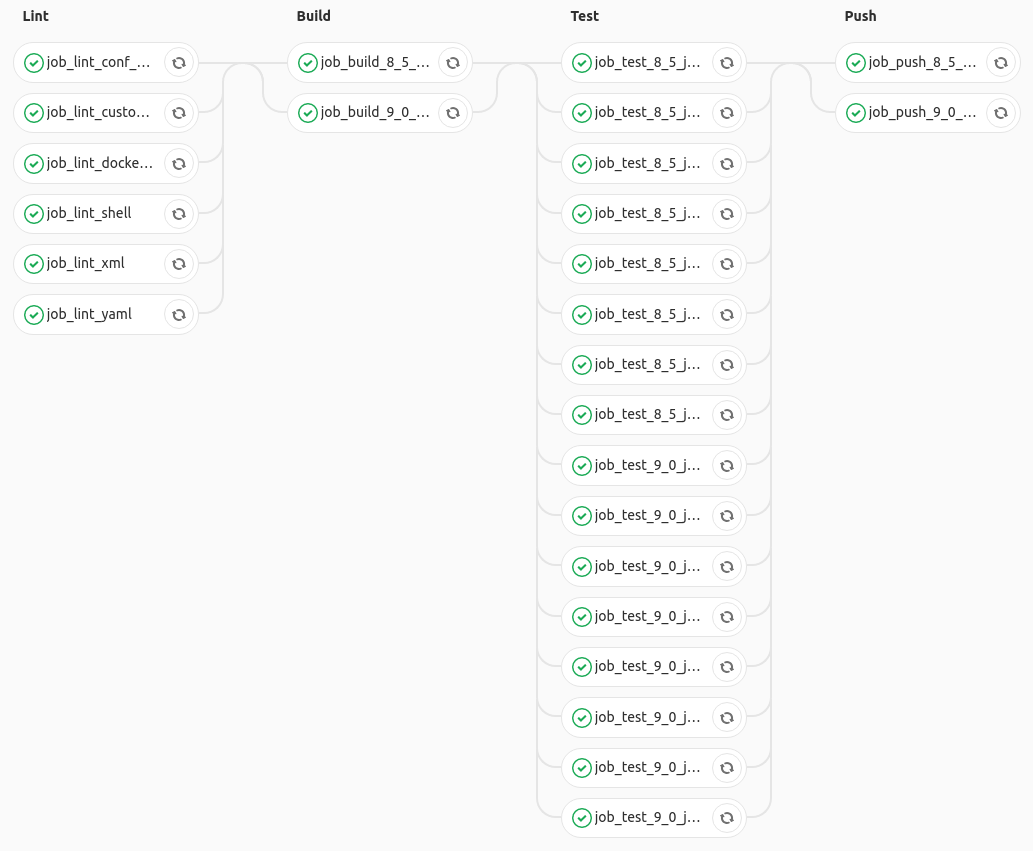
\includegraphics[height=0.9\textheight]{images/pipeline_multi.png}
  \end{figure}
\end{frame}

\section{Future Improvements}

\subsection{Explore non-DinD options}

\begin{frame}
  \frametitle{Explore non-DinD options}
TODO/TOremove
\end{frame}

\subsection{ContainerStructureTest}

\begin{frame}
  \frametitle{Google's "ContainerStructureTest"}
  \begin{itemize}
    \item Recent Google tool similar to Goss
    \item Basic tests runnable \textbf{without} Docker daemon (!)
    \item Not as featurerich, but will likely receive more support
  \end{itemize}
\end{frame}

\subsection{Clair}

\begin{frame}
  \frametitle{Clair}
TODO/TOremove
\end{frame}


\section{}

\cernSplashWhite

\end{document}
